\documentclass[border=10pt]{standalone}
\usepackage{tikz}
\usetikzlibrary{arrows.meta,positioning,calc,decorations.pathmorphing}
\usepackage{amsmath,amssymb}

\begin{document}
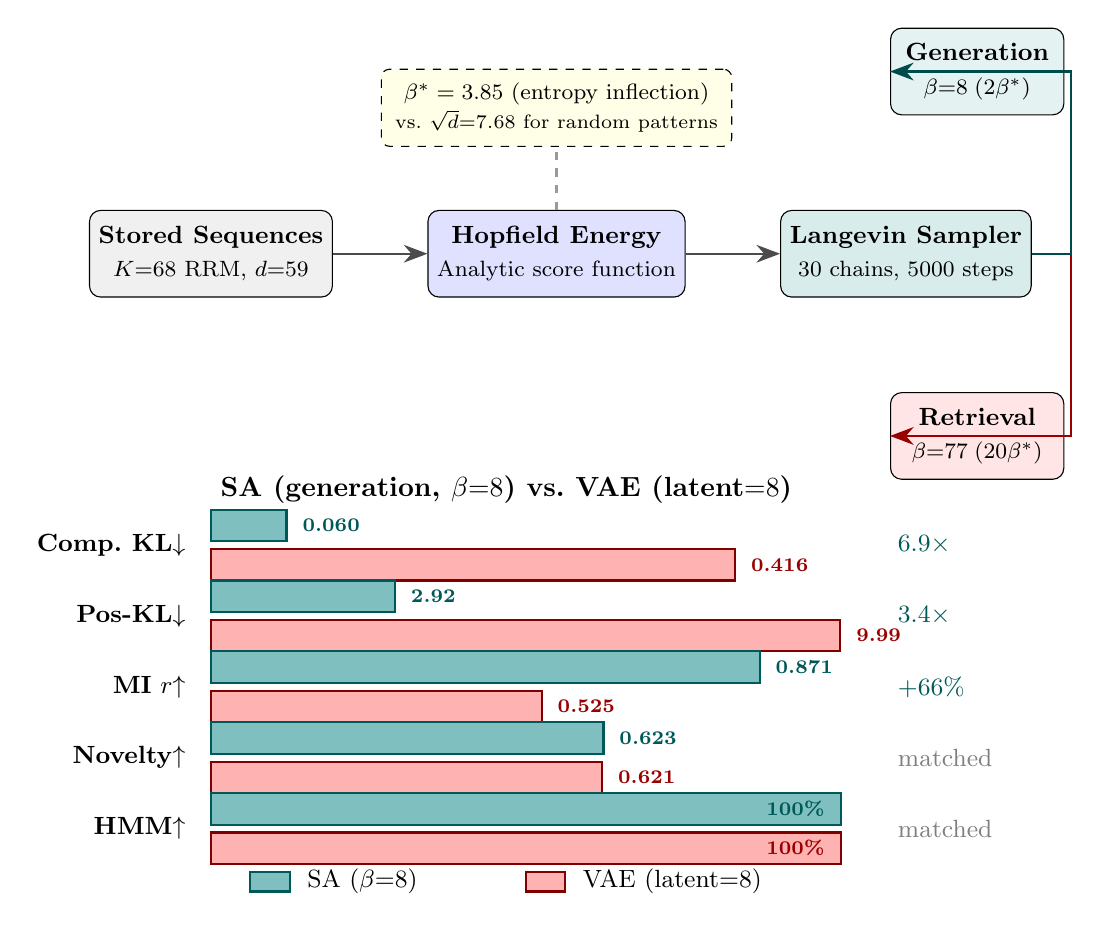
\begin{tikzpicture}[
    block/.style={rectangle, draw, rounded corners=4pt, minimum height=1.1cm, align=center, font=\small},
    arr/.style={-{Stealth[length=3mm]}, thick},
]

% ============================================================
% TOP: Pipeline schematic (horizontal flow)
% ============================================================

% Stored sequences
\node[block, fill=gray!12, minimum width=2.8cm] (stored) {
    \textbf{Stored Sequences}\\[1pt]
    {\footnotesize $K{=}68$ RRM, $d{=}59$}
};

% Hopfield energy
\node[block, fill=blue!12, minimum width=2.8cm, right=1.2cm of stored] (energy) {
    \textbf{Hopfield Energy}\\[1pt]
    {\footnotesize Analytic score function}
};

% Langevin sampler
\node[block, fill=teal!15, minimum width=2.8cm, right=1.2cm of energy] (sampler) {
    \textbf{Langevin Sampler}\\[1pt]
    {\footnotesize 30 chains, 5000 steps}
};

% Arrows
\draw[arr, black!70] (stored) -- (energy);
\draw[arr, black!70] (energy) -- (sampler);

% Beta* annotation above energy
\node[draw, dashed, rounded corners=3pt, fill=yellow!10, font=\footnotesize,
      above=0.8cm of energy, align=center, inner sep=5pt] (inflection) {
    $\beta^* = 3.85$ (entropy inflection)\\[1pt]
    {\scriptsize vs.\ $\sqrt{d}{=}7.68$ for random patterns}
};
\draw[dashed, black!40, thick] (energy.north) -- (inflection.south);

% Two output branches from sampler
\node[block, fill=red!10, minimum width=2.2cm, below right=1.2cm and -1.8cm of sampler] (retrieval) {
    \textbf{Retrieval}\\[1pt]
    {\footnotesize $\beta{=}77\;(20\beta^*)$}
};
\node[block, fill=teal!10, minimum width=2.2cm, above right=1.2cm and -1.8cm of sampler] (generation) {
    \textbf{Generation}\\[1pt]
    {\footnotesize $\beta{=}8\;(2\beta^*)$}
};

\draw[arr, red!60!black] (sampler.east) -- ++(0.5,0) |- (retrieval.west);
\draw[arr, teal!60!black] (sampler.east) -- ++(0.5,0) |- (generation.west);

% ============================================================
% BOTTOM: Grouped bar chart (vertical layout, below pipeline)
% ============================================================

\def\chartx{0.0}
\def\charty{-3.5}
\def\barh{0.20}
\def\gap{0.05}
\def\maxbar{8.0}    % max bar length

% Title
\node[font=\normalsize\bfseries, anchor=west] at (\chartx, \charty+0.5) {SA (generation, $\beta{=}8$) vs.\ VAE (latent${=}8$)};

% --- Metric 1: Global KL ---
\def\mone{\charty-0.2}
\node[font=\small, anchor=east] at (\chartx-0.2, \mone) {\textbf{Comp.\ KL}$\downarrow$};
% SA bar (0.060/0.5 * maxbar = 0.96)
\fill[teal!50] (\chartx, \mone+\gap) rectangle (\chartx+0.96, \mone+\gap+2*\barh);
\draw[thick, teal!70!black] (\chartx, \mone+\gap) rectangle (\chartx+0.96, \mone+\gap+2*\barh);
\node[font=\scriptsize\bfseries, teal!70!black, anchor=west] at (\chartx+0.96+0.08, \mone+\gap+\barh) {0.060};
% VAE bar (0.416/0.5 * maxbar = 6.656)
\fill[red!30] (\chartx, \mone-\gap-2*\barh) rectangle (\chartx+6.656, \mone-\gap);
\draw[thick, red!50!black] (\chartx, \mone-\gap-2*\barh) rectangle (\chartx+6.656, \mone-\gap);
\node[font=\scriptsize\bfseries, red!60!black, anchor=west] at (\chartx+6.656+0.08, \mone-\gap-\barh) {0.416};
% Improvement
\node[font=\small\bfseries, teal!70!black, anchor=west] at (\chartx+\maxbar+0.6, \mone) {$6.9\times$};

% --- Metric 2: Per-position KL ---
\def\mtwo{\charty-1.1}
\node[font=\small, anchor=east] at (\chartx-0.2, \mtwo) {\textbf{Pos-KL}$\downarrow$};
% SA bar (2.92/10 * maxbar = 2.336)
\fill[teal!50] (\chartx, \mtwo+\gap) rectangle (\chartx+2.336, \mtwo+\gap+2*\barh);
\draw[thick, teal!70!black] (\chartx, \mtwo+\gap) rectangle (\chartx+2.336, \mtwo+\gap+2*\barh);
\node[font=\scriptsize\bfseries, teal!70!black, anchor=west] at (\chartx+2.336+0.08, \mtwo+\gap+\barh) {2.92};
% VAE bar (9.99/10 * maxbar = 7.992)
\fill[red!30] (\chartx, \mtwo-\gap-2*\barh) rectangle (\chartx+7.992, \mtwo-\gap);
\draw[thick, red!50!black] (\chartx, \mtwo-\gap-2*\barh) rectangle (\chartx+7.992, \mtwo-\gap);
\node[font=\scriptsize\bfseries, red!60!black, anchor=west] at (\chartx+7.992+0.08, \mtwo-\gap-\barh) {9.99};
% Improvement
\node[font=\small\bfseries, teal!70!black, anchor=west] at (\chartx+\maxbar+0.6, \mtwo) {$3.4\times$};

% --- Metric 3: MI correlation ---
\def\mthree{\charty-2.0}
\node[font=\small, anchor=east] at (\chartx-0.2, \mthree) {\textbf{MI}~$r$$\uparrow$};
% SA bar (0.871 * maxbar = 6.968)
\fill[teal!50] (\chartx, \mthree+\gap) rectangle (\chartx+6.968, \mthree+\gap+2*\barh);
\draw[thick, teal!70!black] (\chartx, \mthree+\gap) rectangle (\chartx+6.968, \mthree+\gap+2*\barh);
\node[font=\scriptsize\bfseries, teal!70!black, anchor=west] at (\chartx+6.968+0.08, \mthree+\gap+\barh) {0.871};
% VAE bar (0.525 * maxbar = 4.2)
\fill[red!30] (\chartx, \mthree-\gap-2*\barh) rectangle (\chartx+4.2, \mthree-\gap);
\draw[thick, red!50!black] (\chartx, \mthree-\gap-2*\barh) rectangle (\chartx+4.2, \mthree-\gap);
\node[font=\scriptsize\bfseries, red!60!black, anchor=west] at (\chartx+4.2+0.08, \mthree-\gap-\barh) {0.525};
% Improvement
\node[font=\small\bfseries, teal!70!black, anchor=west] at (\chartx+\maxbar+0.6, \mthree) {$+66\%$};

% --- Metric 4: Novelty ---
\def\mfour{\charty-2.9}
\node[font=\small, anchor=east] at (\chartx-0.2, \mfour) {\textbf{Novelty}$\uparrow$};
% SA bar (0.623 * maxbar = 4.984)
\fill[teal!50] (\chartx, \mfour+\gap) rectangle (\chartx+4.984, \mfour+\gap+2*\barh);
\draw[thick, teal!70!black] (\chartx, \mfour+\gap) rectangle (\chartx+4.984, \mfour+\gap+2*\barh);
\node[font=\scriptsize\bfseries, teal!70!black, anchor=west] at (\chartx+4.984+0.08, \mfour+\gap+\barh) {0.623};
% VAE bar (0.621 * maxbar = 4.968)
\fill[red!30] (\chartx, \mfour-\gap-2*\barh) rectangle (\chartx+4.968, \mfour-\gap);
\draw[thick, red!50!black] (\chartx, \mfour-\gap-2*\barh) rectangle (\chartx+4.968, \mfour-\gap);
\node[font=\scriptsize\bfseries, red!60!black, anchor=west] at (\chartx+4.968+0.08, \mfour-\gap-\barh) {0.621};
% Annotation
\node[font=\small, black!50, anchor=west] at (\chartx+\maxbar+0.6, \mfour) {matched};

% --- Metric 5: HMM pass ---
\def\mfive{\charty-3.8}
\node[font=\small, anchor=east] at (\chartx-0.2, \mfive) {\textbf{HMM}$\uparrow$};
% SA bar
\fill[teal!50] (\chartx, \mfive+\gap) rectangle (\chartx+\maxbar, \mfive+\gap+2*\barh);
\draw[thick, teal!70!black] (\chartx, \mfive+\gap) rectangle (\chartx+\maxbar, \mfive+\gap+2*\barh);
\node[font=\scriptsize\bfseries, teal!70!black, anchor=east] at (\chartx+\maxbar-0.08, \mfive+\gap+\barh) {100\%};
% VAE bar
\fill[red!30] (\chartx, \mfive-\gap-2*\barh) rectangle (\chartx+\maxbar, \mfive-\gap);
\draw[thick, red!50!black] (\chartx, \mfive-\gap-2*\barh) rectangle (\chartx+\maxbar, \mfive-\gap);
\node[font=\scriptsize\bfseries, red!60!black, anchor=east] at (\chartx+\maxbar-0.08, \mfive-\gap-\barh) {100\%};
% Annotation
\node[font=\small, black!50, anchor=west] at (\chartx+\maxbar+0.6, \mfive) {matched};

% Legend
\fill[teal!50] (\chartx+0.5, \charty-4.6) rectangle (\chartx+1.0, \charty-4.35);
\draw[thick, teal!70!black] (\chartx+0.5, \charty-4.6) rectangle (\chartx+1.0, \charty-4.35);
\node[font=\small, anchor=west] at (\chartx+1.1, \charty-4.475) {SA ($\beta{=}8$)};

\fill[red!30] (\chartx+4.0, \charty-4.6) rectangle (\chartx+4.5, \charty-4.35);
\draw[thick, red!50!black] (\chartx+4.0, \charty-4.6) rectangle (\chartx+4.5, \charty-4.35);
\node[font=\small, anchor=west] at (\chartx+4.6, \charty-4.475) {VAE (latent${=}8$)};

\end{tikzpicture}
\end{document}
